%*****************************************
\chapter{Research Field}\label{ch:research}
%*****************************************
In der Arbeitswelt kommt es immer wieder zu Situationen, in der sich mehrere Personen treffen um zusammen Probleme zu diskutieren. Statistiken besagen, dass Büroangestellte sogar bis zu 70 Prozent ihrer Arbeitszeit in Meetings verbringen \citep{panko:1993}. Die meisten Meetings werden mit Hilfsmittel wie Whiteboards, Flipcharts oder Notizblöcke abgehalten, da meistens Notierungsbedarf bei neuen Ideen, Problemlösungen etc. besteht. Computer können dabei sehr hilfreich sein, wäre da nicht die Hürde der Dateneingabe die zu bewältigen ist. Herkömmliche Eingaben via Maus und Tastatur verlangsamen den natürlichen explorativen Charakter eines Meetings. Elektronische Skizzierwerkzeuge inklusive gemeinsam verwendbarer Zeichenoberflächen können hier Abhilfe für kollaboratives Arbeiten schaffen. 

\medskip Das folgende Kapitel soll anhand von Beispielen und Projekten aus der Literatur zeigen, durch welche Methoden Meetings bzw. im speziellen Designsessions unterstützt werden können. Besonderer Augenmerk soll dabei auf das Skizzieren als Designmethode und kooperatives Arbeiten in CSCW\footnote{Computer Supported Cooperative Work} Umgebungen liegen.

\section{Arbeitsweisen von Designteams}
Um herauszufinden mit welchen Methoden oder Werkzeugen man kollaborative Meetings und im Zuge dessen den Designprozess unterstützen kann, muss man zuerst wissen wie Designer zusammen arbeiten. John Tang und Larry Leifer versuchten in \citep{Tang:1988p279} als Teil einer Studie, mittels empirischen Daten das Verhalten von Designern in Meetings zu untersuchen. Dazu bildeten sie ein Framework und konzentrierten sich auf deren Arbeitsaktivitäten wie \emph{Auflisten}, \emph{Zeichnen} und \emph{Gestikulieren}, welche sie den zugehörigen Kontext zuordneten. Um diesen einzuschränken, bildeten sie vier Funktionen, die den Hauptzweck der Aktivitäten beschreiben: \emph{Festhalten von Informationen}, \emph{Vermitteln von Ideen}, \emph{Darstellen von Ideen} und \emph{Erlangen von Aufmerksamkeit}. In einem Framework (siehe \autoref{fig:TangFramework}) stellten sie diese gegenüber und verwendeten die Daten zur Auswertung.

\medskip Obwohl sich Tang und Leifer mit ihrer Arbeit gezielt auf den Designprozess zubewegen, erwarten sie dadurch auch relevante Ergebnisse für kollaboratives Arbeiten im Allgemeinen. \par Kollaboratives Arbeiten ist für Designer eine gängige Art Probleme anzugehen und kann von den sonstigen individuellen Aktivitäten deutlich abgegrenzt werden, wie auch frühere empirische Designstudien bestätigen können (\citep{Ullman:1987}, \citep{Ballay:1987}, \citep{Akin:1978}, \citep{Lera:1983}).
In ihrer Studie führten sie 8 Sessions mit Teams zu je 3-4 Personen durch, welche jeweils eineinhalb Stunden dauerten. Die Gruppen trafen sich dafür in Konferenzräumen und saßen um einen Tisch mit einem großen Bogen Papier als Schreibunterlage. Jede Gruppe arbeitete zwar an einer anderen Designaufgabe, jedoch waren alle Teil des Designs eines Mensch-Maschinen Interfaces für ein >>smartes<< (Mikroprozessor gesteuertes) Gerät.
Die Analyse der Tests wurde durch das NoteCards Hypertext Environment \citep{Halasz:1986:NN:29933.30859} erheblich vereinfacht. Das System half die Daten zu strukturieren und aufzubereiten. \autoref{fig:TangTranskript} zeigt einen Auszug des Transkripts der ersten Session mit Anmerkungen zu einzelnen Aktivitäten und einen Teil der Schreibunterlage, welche die dazu erstellte Skizze beinhaltet. Jede Aktivität wurde anhand der Funktionen des Frameworks kategorisiert und abgezählt, um in Folge dessen die Daten statistisch auszuwerten. \autoref{fig:TangStatistik} veranschaulicht die Ergebnisse.

\medskip Wie die Abbildung zeigt, sind knapp die Hälfte (46\%) aller Aktivitäten von illustrativen Charakter, was die Wichtigkeit von Skizzen belegt. Zusätzlich kommt der Vermittlung und Darstellung von Ideen (zusammen 43\%) auch große Bedeutung zu.\par
\medskip \emph{Anmerkung: An diesem Punkt der Arbeit soll noch nicht auf die gesamten Erkenntnisse der Analyse eingegangen werden, sondern lediglich auf die der Ideenentwicklung. Die weiteren Ergebnisse werden in den Kapitel >>Single VS Group Design<< und >>CSCW \& Design<< behandelt.}

\medskip Die Schreibunterlage spielt im Prozess der Ideenentwicklung, neben der des Festhaltens von Informationen und der Vermittlung von Ideen, eine aktive Rolle. Die Unterstützung dieses Prozesses (zb. durch elektronische Hilfsmittel) ist aber alles andere als unproblematisch, wie beispielsweise die Frustrationen von Designer beweisen, die versuchen konventionelle CAD Tools für die Weiterentwicklung von Ideen - von konzeptionellen Skizzen zu formellen Spezifikationen - zu verwenden. Dieser Aspekt zeigt die Verwendung der Schreibunterlage als Teil eines interaktiven Prozesses, anstatt der Reduzierung dessen auf ein Text-Grafik Artefakt. 
Die Studie beobachtete 2 Schlüsselmerkmale, auf die Designer bei der Entwicklung von Ideen zurückgriffen: a) In der Lage sein ohne Weiteres Darstellungen von Ideen auf einer Schreibunterlage auszuprobieren, und b) diese Darstellungen stufenweise in genaue Artefakte weiterzuverarbeiten - oft durch die Zusammenarbeit mit anderen Partizipienten. \citep{Tang:1988p279}

%\clearpage
\begin{figure}
        {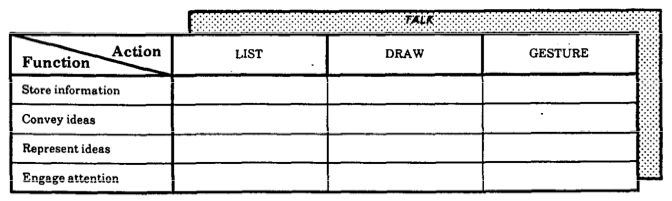
\includegraphics[width=1\linewidth]{gfx/Abb1}}
		\caption[Framework zur Untersuchung von Designaktivitäten.]{Das Framework zur Untersuchung von Designaktivitäten. In ihm werden die Aktivitäten den zweckmäßigen Funktionen gegenübergestellt. Es dient als empirische Grundlage. }\label{fig:TangFramework}
\end{figure} 

\begin{figure}[bth]
        \myfloatalign
        \subfloat[Transkriptauszug]
        {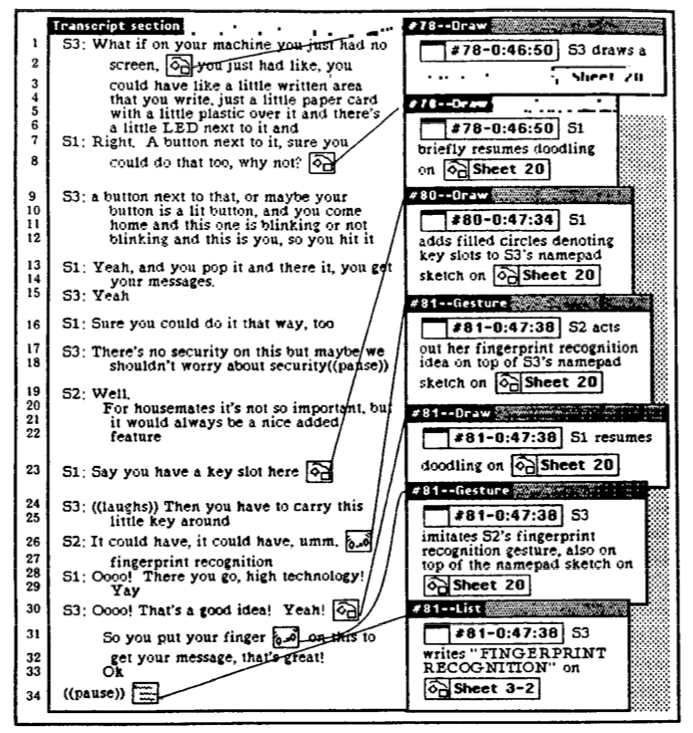
\includegraphics[width=.65\linewidth]{gfx/Abb2_1}} \quad
        \subfloat[Artefakt]
        {\label{fig:TangTranskriptB}%
         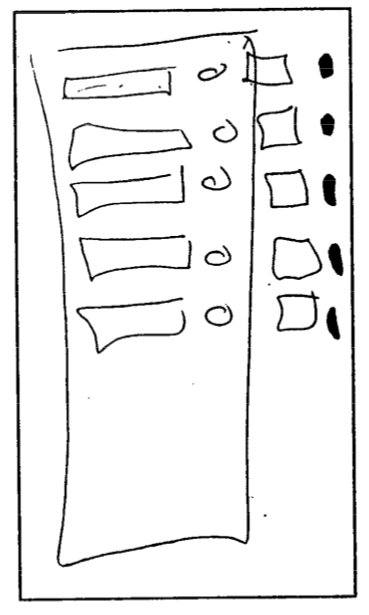
\includegraphics[width=.25\linewidth]{gfx/Abb2_2}} \\
        \caption[Auszug des Transkripts inklusive dazugehöriges angefertigtes Artefakt der ersten Designsession.]{Ein Auszug des Transkripts, erstellt mit Hilfe von NoteCards \citep{Halasz:1986:NN:29933.30859}, inklusive dazugehörigen  Artefakt der ersten Designsession. Es zeigt wie jeder Teilnehmer in kürzester Zeit einen eigenen Gedanken äußert und diesen im Artefakt manifestiert.}\label{fig:TangTranskript}
\end{figure}

\begin{figure}
        {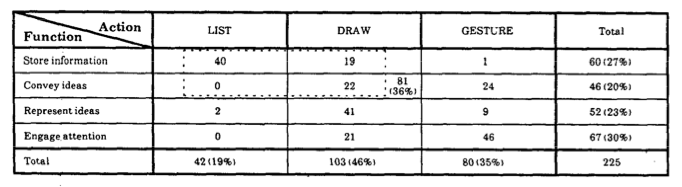
\includegraphics[width=1\linewidth]{gfx/Abb3}}
		\caption[Statistische Ergebnisse der ersten Designsession.]{Statistische Ergebnisse der ersten Designsession. Alle Aktivitäten wurden dafür im Framework anhand der Funktionen kategorisiert und anschließend abgezählt.}\label{fig:TangStatistik}
\end{figure}
\clearpage

\medskip Gemeinsam verwendbare Zeichenoberflächen spielen auch laut Sara Bly \citep{Bly:1988:UDS:62266.62286} eine besonders wichtige Rolle in Designsessions mit mehreren Teilnehmern. 
Bly beobachtete das Skizzierverhalten zweier Personen in Face-to-Face Designsessions und zeichnete diese für spätere Anaylsen auf Video auf. Bei der Auswertung stellte sie fest, dass nahezu die Hälfte aller Aktivitäten, in denen Gebrauch von Schreibwerkzeugen gemacht wurde, Skizzen waren. Noch interessanter war aber die Tatsache, dass sich im Laufe der Session verschiedene Zeichenbereiche herauskristallisiert haben. So entstanden einzelne Bereiche in denen nur ein Designer gezeichnet hat und Bereiche die zusammen benutzt wurden. 78\% aller Aktivitäten fanden jedoch im gemeinsamen Bereich statt und 25\% aller Aktivitäten eines Designers entstanden im Anschluss zu einer Zeichnung eines anderen Designers. Die Analyse zeigt also die Wichtigkeit von gemeinsamen Bereichen in Designsessions mit mehreren Teilnehmern. Zusätzlich spielten Gesten und Betonungen in Erläuterungen eine wichtige Rolle, welche die Notwendigkeit der physischen Anwesenheit nahelegt.

\section{Skizziertools in kooperativen Settings}
Dies als Ansporn und Grundlage für weitere Arbeiten nahm sich das Department of Computer Science auf der Universität in Toronto und entwickelte XSketch: ein Multiuser Skizzierwerkzeug für X11\footnote{X11 ist ein Softwaresystem für UNIX Plattformen, dass ein Grafisches User Interface (GUI) zur Verfügung stellt - auch bekannt als X-Windows.}, dass Jefferey J. Lee bereits 1990 in \citep{Lee:1990:XMS:91478.91510} vorstellt und dessen Eigenschaften ich folgend kurz beschreiben will.
Die Grundidee von XSketch ist ein simples Werkzeug für Multiuser Design- und Brainstormingsessions bereitzustellen. Da es aber auch für einzelne Benutzer geeignet sein soll, hat der Multiuserfaktor nur wenig Einfluss auf das User Interface. Es setzt auf eine Server-Client Architektur, in der alle Nachrichten und Entscheidungen zentral gesteuert werden und Benutzer via TCP/IP Protokoll kommunizieren. Das Zeichenmodell kann man mit einem Notizblock oder Flipchart vergleichen, in dem Benutzer auf leeren Seiten zeichnen und zwischen mehreren Seiten hin und her >>blättern<< können. Zeichnungen basieren auf ein objektorientierten Ansatz, sodass man leicht ganze Objekte ausschneiden und kopieren kann. Den Benutzern stehen Polylinien\footnote{Polylinien sind eine Aneinanderreihung von Linien. In der Computergrafik werden sie zur Annäherung an Kurven benutzt.}, Rechtecke und simpler Text als Objekte zur Verfügung. Die Interaktion basiert dabei hauptsächlich auf Mauseingaben, die Tastatur wird lediglich zur Eingabe und Änderung von Texten und Dateinamen verwendet. Die meisten Editieroperationen sind ebenfalls an die Mausbuttons gebunden. 
Mit dem Vorsatz das Interface so schlicht wie möglich zu halten, existieren relativ wenig Modi und keine Möglichkeit Attribute wie Linienart, -stärke, Pfeilspitzen etc. zu ändern. Dafür ist es möglich einen Telepointer durch Druck auf eine bestimmte Maustaste einzublenden, um so das Gezeichnete für die anderen Benutzer hervorheben zu können. Diese Funktion soll als Ersatz für Gesten dienen.
Die einzige Multiuser-Funktion ist der >>Invite Button<<, der dazu benutzt werden kann um anderen Benutzern Nachrichten zu schicken und sie zu einer Session einzuladen. Nehmen diese teil, können sie alle Objekte ändern, nicht nur die eigenen. Ansonsten unterscheidet sich eine Multi-User Session kaum von einer Single-User Session.

\medskip Obwohl der Prototyp von XSketch allen anfänglichen Zielen und Anforderungen der Projektgruppe entspricht, gibt es nach Lees Erfahrungen in einigen Fällen Verbesserungspotenzial. So wirkt z.B. das Zeichnen von Skizzen unbefriedigend. Ein möglicher Lösungsansatz für dieses Problem wäre, neue grafische Objekte wie Ellipsen oder Splines zur Objektauswahl hinzuzufügen und das Einfügen von Bitmapbildern zu erlauben, um so das Repertoire an Tools aufzustocken. \graffito{Ein gutes Multi- User Skizzier Programm benötigt eine große Auswahl an Tools oder sollte sich durch und durch auf Freihandzeichnungen beschränken.} Im Gegensatz dazu könnte man das Repertoire aber auch verringern und durch und durch auf reine Freihandzeichnungen setzen. Welcher der bessere Ansatz wäre, müsse ausprobiert werden.
Ein weiterer verbesserungsbedürftiger Punkt ist das strikte Cut\&Paste Modell. Eigentlich anfangs bewusst dafür entschieden um Kollisionen im Datenmanagement vorzubeugen, steht das Entwicklungsteam dadurch vor Usabilityproblemen. Durch die Tatsache, dass man existierende Objekte nicht nachträglich ändern kann, entsteht Frust bei den Benutzern. Ein optimistisches Sperrmodell\footnote{Sperrmodelle in der elektronischen Datenverarbeitung sind Mechanismen die Datenbankressourcen sperren, um zu verhindern, dass mehrere Datenzugriffe gleichzeitig stattfinden können. Man unterscheidet zwischen optimistischen und pessimistischen Sperrstrategien. Eine pessimistische Sperrstrategie schützt die Integrität der Datenbank, indem Datenbankressourcen während der gesamten Dauer einer Transaktion von Anfang bis Ende gesperrt werden. Eine optimistische Sperrstrategie hingegen senkt die Isolationsstufe, so dass weniger Sperren auf die Datenbankressourcen angewandt werden. Auf diese Weise können mehr Anwendungen gleichzeitig auf eine Datenbank zugreifen, was den Durchsatz potenziell erhöhen kann. \citep{IBM:1996:Online}} könnte, im Gegensatz zu konventionellen zentralisierten (pessimistischen) Sperrmodellen, das Selektieren und nachträgliche Ändern von Objekten ohne lästige Verzögerung ermöglichen. \graffito{Nachträgliches Ändern von Skizzen und eine dazugehörige Undo- Funktion sind wünschenswert.}Erstrebenswert wäre diesbezüglich auch eine dazugehörige Undo Funktion, welche die derzeitige Pseudo-Undo Funktion mittels Löschen ersetzt.
Wie auch schon Bly feststellte, ist in einer Designsession mit mehreren Teilnehmern der Prozess des Zeichnens für den Designprozess genau so wichtig wie die Zeichnungen selbst. \citep{Bly:1988:UDS:62266.62286} Aus diesem Grund ist es wichtig, dass alle Teilnehmer sehen können was die anderen machen. \graffito{Alle Teilnehmer müssen stets über die Tätigkeiten der anderen im Bilde sein.}Leider können Benutzer von XSketch nicht sehen, wenn andere Benutzer Objekte erstellen oder selektieren, da der Vorgang bis zu seinem Abschluss rein lokal abläuft. Diese Entscheidung ist laut Lee schlichtweg ein Fehler und muss unbedingt ausgebessert werden. Ebenso das Ausbleiben einer Möglichkeit um untereinander kommunizieren zu können, sieht er als Fehlgriff, da es im geplanten Setting oft vorkommt dass viele User in einem großen Raum verteilt sitzen und kein Telefon bei sich haben um erreichbar zu sein. Hier wäre eine integrierte Nachrichtenfunktion im Programm denkbar, wie z.B. auch in MUSK \citep{Crampton:1987} umgesetzt wurde. Das würde den Benutzern zusätzlich helfen eine Übersicht über alle Teilnehmer zu bekommen. 
Schließlich, resümiert Lee, war es rückblickend auch falsch anzunehmen, dass sich die Anforderungen von Multi-User Systemen von Single-User Systemen nicht unterscheiden. Der Prototyp wurde in simplen Designsessions mit einem, zwei und drei Benutzer(n) getestet und zeigte zwar über eine 19,2Kbaud Verbindung eine gute Performance, jedoch beschränken die oben genannten \graffito{Ein Grafiktablet in Verbindung mit einem Flatscreen wäre ein ideales Setting für ein Multi- User Skizziertool.}Probleme den Einsatz noch auf Institutsexperimente.
Unglücklicherweise zeigten die Tests auch, dass ein Maus basierendes System für interaktive Skizziersessions nicht ideal ist. Ein ideales Interface für diese Art von Programm wäre laut Lee ein gut integriertes Grafiktablet in Verbindung mit einem Flatscreen. Das wäre die bestmögliche Annäherung zu einer Technologie, die Stift und Papier ersetzen könne.

\bigskip Tangs und Blys Observationen animierten auch Greenberg et al. \emph{Group Drawing Tools} zu erstellen. In \citep{Greenberg:1992p83} beschreiben sie die Probleme und Erfahrungen die sie mit dem Design von zwei Systemen gemacht haben, die realtime Online Gruppenarbeit ermöglichen: \emph{GroupSketch}, ein Multiuser Skizziertool; und \emph{GroupDraw}, ein objektbasiertes Multiuser Zeichenpaket.

\medskip \emph{GroupSketch} ist ein simples Gruppenskizziertool, das einer beliebigen Anzahl an Teilnehmern ermöglicht auf einem virtuellen Blatt Papier (dem Bildschrirm) zu zeichnen \citep{Greenberg:1991}. Zu seinen Hauptmerkmalen zählen:
\begin{itemize}
	\item{ein What-You-See-Is-What-I-See (WYSIWIS) Bildschirm}
	\item{multible, aktive Curor, die alle Teilnehmer identifizieren und stets sichtbar sind}
	\item{unterstützte gleichzeitige Interaktion, sodass jeder Teilnehmer zu jeder Zeit arbeiten kann}
	\item{Benutzeraktionen (Cursorbewegung oder Zeichnung), egal wie klein, sind sofort auf allen Screens sichtbar}
	\item{Zeichnen, Gestikulieren und Auflisten sind so einfach wie möglich umgesetzt (Benutzer müssen keine eigenen Modi auswählen)}
\end{itemize}

\autoref{fig:GroupSketch} zeigt einen typischen Groupsketch Screen mit vier Teilnehmern einer Designsession. Auf der linken Seite befindet sich die gemeinsam benutzbare Zeichenfläche, in der die Benutzer zeichnen, schreiben oder gestikulieren können. Jede Person hat einen eigenen Cursor, der mit seinem Namen versehen ist. 

\begin{figure}
        {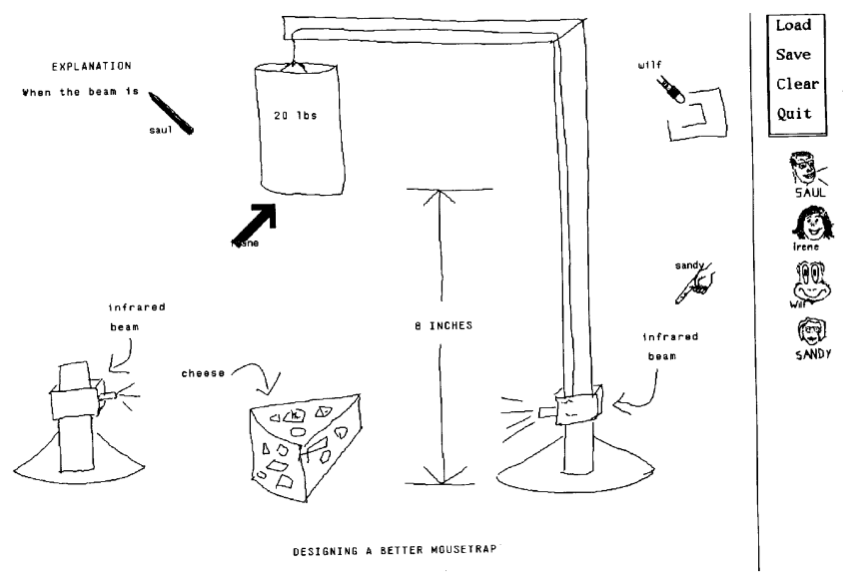
\includegraphics[width=1\linewidth]{gfx/GroupSketch}}
		\caption[GroupSketch]{Eine typische GroupSketch Session mit 4 Teilnehmer. Sie zeigt die Grundfunktionen..}\label{fig:GroupSketch}
\end{figure}

\section{Communication and Information Retrieval with a Pen-based Meeting Support Tool}
Das Paper befasst sich mit dem prototypisch implementierten Meeting Support Tool \emph{We-Met}. Dieses verwendet ein stiftbasiertes Interface, das durch das Skizzieren der Benutzer auf digitale Medien, die Kommunikation während Meetings fördern und die nachträgliche Auswertung der angefertigten Zeichnungen erleichtern soll.

\subsection{We-Met}
\emph{We-Met} \citep{Wolf:1997p75} kann bei face-to-face Meetings, als auch bei geographisch distanzierten Meetings zusammen mit einer Telefonkonferenz eingesetzt werden. Jeder Teilnehmer benötigt einen Computer mit einem Bildschirm und einem stiftbasierten Eingabetablett. Die Geräte werden über ein lokales LAN Netzwerk verbunden. Das Interface bietet mehrere gemeinsame Bereiche für Skizzen und Zeichnungen, die nach jedem vollendeten Strich eines Benutzers aktualisiert werden. Somit sehen alle Teilnehmer die Zeichnungen der anderen nahezu in Echtzeit.

Alle Meetings werden aufgezeichnet und können während dessen oder nach Abschluss der Sitzung aufgearbeitet werden. Jeder Zeichenstrich wird mit einem Zeitstempel versehen, sodass der Zeichenprozess Schritt für Schritt vor- und zurückgespult werden kann. Außerdem erlaubt \emph{We-Met} bestimmte zeitliche und räumliche Zustände der Skizzen mit Tags\footnote{Unter einem \emph{Tag} versteht man ein Schlagwort, das der Kategorisierung, bzw. Thematisierung eines bestimmten Datenbestands dient.} zu versehen, sodass sie leichter zwischen diesen hin und her springen können. Die Form der Tags ist an Markierungen angelehnt, die Personen auch in ihren echten Notizbüchern verwenden, denn sie können nicht nur aus Textelementen, sondern auch aus handgezeichneten Schnörkeln, Kügelchen oder Sternchen bestehen, wodurch das Anlegen von Tags einfacher und intuitiver wird.

\subsection{Studie: We-Met als Tool zur Kommunikation in Gruppen}
Schon während der Entwicklung von Prototypen ist es wichtig, das Konzept so früh wie möglich zu testen und zu evaluieren. \emph{We-Met} wurde daher schon sehr bald in einer Studie mit potenziellen Nutzern getestet. Die Entwickler zogen drei Gruppen mit je drei Teilnehmern und eine Gruppe mit zwei Teilnehmern heran. Die Testpersonen erhielten die Aufgabe unter Gebrauch von \emph{We-Met} einen Haushaltsroboter zu konzipieren, der Müll aufsammelt und in einen dafür vorgesehenen Behälter wirft. Viel mehr, als ein finales Design zu schaffen, ging es darum, möglichst viele Ideen zu generieren und zu skizzieren.

\subsubsection{Resultate}
\begin{itemize}
	\item \textit{Einfacher Zugang durch stiftbasiertes Interface}\\
	Alle Teilnehmer empfanden das stiftbasierte Interface einfach zu benutzen. Es fiel ihnen nicht schwer, während dem Schreiben und Kritzeln der Diskussion zuzuhören und sich aktiv daran zu beteiligen. Das Arbeiten mit einer Tastatur hingegen, erfordert bei vielen Personen einen zu hohen kognitiven Aufwand, um einer Diskussion noch mit ausreichender Aufmerksamkeit beiwohnen zu können. Aufgrund dieser Tatsache hat das stiftbasierte Interface das Potenzial, die Produktivität eines solchen Meetings zu erhöhen, denn es erlaubt den Teilnehmern die parallele Durchführung mehrerer Aktivitäten.
	
	Die Testpersonen sprachen, zeichneten, schrieben, gestikulierten eifrig und hielten viel Augenkontakt während der Diskussion, ähnlich wie in herkömmlichen Meetings ohne Unterstützung von Computern. Das stiftbasierte Interface ermöglichte dabei sehr rasche und flüssige Übergänge beim Wechsel zwischen diesen Kommunikationskanälen.
	
	\item \textit{Formen der Interaktion}\\
	Eine der Testgruppen arbeitete in einer höchst kollaborativen Art und Weise zusammen. Häufig definierte eine Person Anforderungen an den Haushaltsroboter und hielt diese handschriftlich fest, während eine andere Person die Anforderungen verfeinerte und Skizzen dazu anfertigte. Interessanterweise wählten diese Form der Interaktion genau jene Teilnehmer, die sich vorher nicht bekannt waren. Alle Gruppen befanden einstimmig, dass es einfacher sei sich in die Diskussion einzubringen, als bei herkömmlichen Meetings in denen Whiteboards eingesetzt werden. Etwas zur Sitzung beizutragen bedeutet normalerweise aufzustehen, zur Tafel zu gehen und jemand anderem den Stift zu nehmen. Die natürliche Hemmschwelle, die dadurch entsteht, entfällt bei \emph{We-Met}, da jeder über einen Computer samt Eingabestift verfügt. Der kreative Prozess der Ideenfindung kann so optimiert werden.
	
	Die zweite Gruppe an Testpersonen wählte eine andere Form der Interaktion. Nach einer anfänglichen, gemeinsamen Diskussion, zeichnete und skizzierte jeder Teilnehmer für sich. Nachdem alle fertig waren, wurden die Ergebnisse hergezeigt und wiederum diskutiert. Die Personen arbeiteten also getrennt parallel. Im weiteren Verlauf der Sitzung kam es auch vor, dass zwei Teilnehmer miteinander diskutierten, während ein Dritter für sich skizzierte. Nachdem die anderen fertig diskutiert hatten, brachte der Dritte seine neuen Ideen ein und zeigte den anderen die angefertigten Skizzen. Durch diese Art der getrennten Parallelität, die \emph{We-Met} ermöglicht, können potenziell mehr Ideen gefunden werden und das Ergebnis des Meetings somit verbessert werden.
	
	Anders als bei den vorhergehenden, ergab sich in der dritten Testgruppe eine moderierte Form der Diskussion. In den ersten fünfzehn Minuten sprachen alle drei Teilnehmer miteinander, aber nur einer schrieb Notizen mit. Diese Person kontrollierte auch die Diskussion. Man kann hier das typische Modell eines Meetings mit Whiteboard erkennen.
	
	\item\textit{Gemeinsames Produkt}\\
	Auf die Frage >>Was gefällt Ihnen an \emph{We-Met}?<<, antworteten Teilnehmer aus allen drei Gruppen, sie würden es gut finden, dass es die Möglichkeit biete, ein gemeinsames Produkt hervorzubringen. Im Vergleich zu herkömmlichen Meetings gäbe es ein besseres Allgemeinverständnis in der Gruppe, wodurch Missverständnisse reduziert würden.
	
	\item\textit{Aufteilung der Arbeitsfläche}\\
	Der getestete Prototyp von \emph{We-Met} bot den Teilnehmern keinen privaten Platz für Skizzen und Zeichnungen. Einige der Testpersonen wünschten sich eine private Arbeitsfläche zur Aufzeichnung diverser Notizen. Sie wollten Skizzen auch zuerst fertigstellen, bevor sie bereit waren, sie den anderen Teilnehmern zu zeigen. Daher kam es vor, dass manche sich fernab vom eigentlichen Geschehen auf dem Canvas einen eigenen Platz für ihre Zeichnungen suchten. Andere Gruppen teilten die Arbeitsfläche auf die Teilnehmer auf, sodass jeder seinen eigenen Platz zum Skizzieren fand. Das Fehlen der privaten Arbeitsfläche könnte dazu führen, dass Ideen nicht mitgeteilt werden, da man sie bereits unfertig herzeigen müsste und ebenso könnten Ideen verloren gehen, die man sich für später notiert hätte.
	
	\item\textit{Koordination zwischen den Teilnehmern}\\
	In keiner der Testgruppen gab es Probleme bei der Koordination und es kam nie vor, dass Teilnehmer aus Versehen versuchten, auf dem selben Bereich der Arbeitsfläche zu zeichnen und sich dadurch in die Quere gekommen wären. Da jeder die Zeichenschritte der anderen Teilnehmer Strich für Strich verfolgen konnte, war jedem immer bewusst wer gerade was zeichnete. Schwierigkeiten der Koordination gab es nur bei zwei Aktionen: wechseln der Szene und scrollen der Arbeitsfläche.
	
	Um zu einer neuen Szene zu wechseln, drückt einer der Teilnehmer auf den >>Neu<< Button, wodurch die neue Szene allen Teilnehmern angezeigt wird. Zum Wechseln zu einer bereits vorhandenen Szene, drückt man auf den >>Szenen<< Button und wählt die gewünschte Szene aus der Liste aller zuvor angelegten Szenen aus. Die Liste der Szenen wird nur der Person angezeigt, die auch den >>Szenen<< Button gedrückt hat.
	
	Es gibt drei Aspekte dieses Szenarios, die das Potenzial haben, die Teilnehmer zu verwirren: das Entscheiden, ob die Szene gewechselt werden soll, das Wechseln der Szene und das Erkennen, dass die Szene soeben gewechselt wurde. Die Entscheidung zum Wechsel wurde erwartungsgemäß meist problemlos durchgeführt: Eine Person teilte den anderen Teilnehmern ihre Intention zum Wechsel mit und wartete auf die Zustimmung der anderen.
	
	Die zweite Aktion, das tatsächliche Wechseln der Szene, führte gelegentlich zu Konfusion. Es kam vor, dass nach dem Einverständnis, die Szene zu wechseln, zwei Benutzer gleichzeitig eine neue Szene anlegten, ohne die Aktion des anderen dabei zu bemerken. Dadurch wurde eine Szene mehr angelegt, als die Gruppe im Sinn hatte. Folglich geschah es, dass die Teilnehmer verwirrt waren, als sie zu einem späteren Zeitpunkt versuchten, zur entsprechenden Szene zurück zu wechseln. In einem konkreten Fall wechselte einer der Teilnehmer fünf mal die Szene, beim Versuch, die gewünschte zu finden. Daraufhin versuchte ein anderer Benutzer, die korrekte Szene zu finden und die damit zusammenhängenden Wechsel führten zu leichtem Frust bei einem dritten Teilnehmer.
	
	Gelegentlich realisierten Benutzer nicht, dass eine Szene gewechselt wurde. Das \emph{We-Met} Konzept sieht zwar vor, für jede Szene einen eindeutigen Namen, bzw. eine eindeutige ID anzuzeigen, aber der Prototyp war zum Testzeitpunkt noch nicht so weit entwickelt, weshalb den Personen weniger Informationen als notwendig angezeigt wurden und Fehlerquellen offen blieben.
	
	Einigen Teilnehmern war nicht ganz klar, dass das Scrolling sich nur auf den eigenen Viewport\footnote{Wenn der Bildschirm zu klein ist um alles darzustellen und Scrollbalken zum Einsatz kommen, dann bezeichnet \emph{Viewport} den aktuell sichtbaren Bereich.} und nicht den der anderen bezieht. Sie erwarteten sich ein ähnliches Verhalten wie beim Szenenwechsel, welcher von einem Teilnehmer für die gesamte Gruppe durchgeführt wurde. Deshalb gab es oft Probleme die Bereiche zu finden, in denen gerade ein anderer Benutzer zeichnete. Den Testpersonen war es auch nicht einfach möglich, auf den Bildschirm eines anderen zu schauen, um sich bei der Suche nach dem gewünschten Bereich zu behelfen. Die Gruppe versuchte zwar, sich gegenseitig weiterzuhelfen, hatte jedoch Schwierigkeiten dabei. Das Konzept des Scrollens bereitet oft schon Probleme, wenn es um single-user Software geht, und im multi-user Softwarebereich scheint sich diese Problematik noch zu verschärfen.
	
	Diese verlorene Zeit beim Koordinieren der Gruppe ist definitiv ein Rückschritt im Ideenfindungsprozess, aber die gesteigerte Effizienz im kreativen Teil der Arbeit ist ein Schritt in die richtige Richtung.
\end{itemize}

\subsubsection{Zusammenfassung}
Die Studie, durchgeführt mit dem Prototypen des \emph{We-Met} stiftbasierten Interfacekonzepts, zeigt deutliche Verbesserungen im Kommunikationsprozess während der kreativen Phase der Ideenfindung. \emph{We-Met} erlaubt verschiedene Formen der Interaktion und ist dadurch sehr flexibel. Neben diesen Vorteilen sind auch sehr konkrete Schwachpunkte des Systems zum Vorschein gekommen. Ein unendlich großer Arbeitsbereich, der auf LCD Monitoren nur stark eingeschränkt dargestellt werden kann, und die Tatsache, dass jeder Benutzer unabhängig scrollen kann, bringt einige Schwierigkeiten in der Gruppenkoordination mit sich.


\section{Team Storm}
\emph{Team Storm} \citep{Hailpern:2007p113} ist ein Groupwaresystem, das die Möglichkeit bietet, parallel an mehreren Ideen zu arbeiten. Es kommt bei Meetings in frühen Konzeptionsphasen zum Einsatz und fördert Kreativität innerhalb der Gruppe. Es konzentriert sich auf das Skizzieren von Ideen und bietet private und gemeinsame Arbeitsflächen, auf denen die Designer arbeiten können.

Das System besteht aus drei Hauptkomponenten: den sogenannten Canvases\footnote{Aus dem Englischen: \emph{Leinwand}. Bezeichnet im Softwarebereich einen Bereich zum Zeichnen.} und den privaten sowie gemeinsamen Arbeitsbereichen. Eine Skizze, bzw. ein Design repräsentiert einen Canvas. Die Benutzer können eine beliebige Anzahl an Skizzen erstellen, dabei verwenden sie entweder Tablet-PCs oder andere stiftbasierte Eingabegeräte. 

Zeichnungen werden durch Icons dargestellt, die beliebig auf der privaten Arbeitsfläche (\autoref{fig:teamStorm}, unteres Fenster) positioniert und skaliert werden können. Diese Darstellung bietet deutliche Vorteile: Designer können Relevanz und Fortschritt selbst definieren und die Skizzen dementsprechend anordnen bzw. skalieren. Durch diese Freiheit können ebenso semantisch verknüpfte Zeichnungen zu Gruppen zusammen geordnet werden. Der Nachteil dieser Methode ist der hohe Platzbedarf auf dem Monitor oder dem Tablet-PC.

Auf der gemeinsamen Arbeitsfläche (\autoref{fig:teamStorm}, oberes Fenster), können Designer ihre Canvases mit den anderen Sitzungsteilnehmern teilen, diskutieren, überarbeiten und organisieren. Dieser Bereich, der für jeden vollständig sichtbar ist, bietet allen Benutzern die selben Möglichkeiten wie der private Arbeitsbereich. \autoref{fig:teamStorm} zeigt im oberen Programmfenster eine exemplarische Anordnung mehrerer Skizzen, die von verschiedenen Designern angefertigt und mit den anderen geteilt wurden. \\

\begin{figure}[bth]
	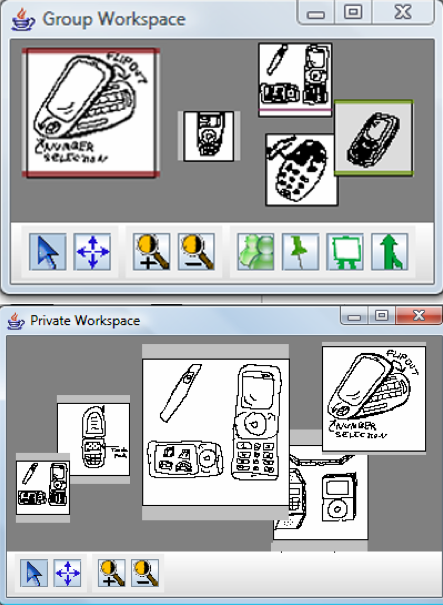
\includegraphics[width=\linewidth]{gfx/teamStormPrivateWorkspace.png}
	\caption{Gemeinsame und private Arbeitsbereiche in \emph{Team Storm}. Designer können ihre Skizzen räumlich anordnen und deren Größe anpassen.}
	\label{fig:teamStorm}
\end{figure}

Während ein Designer eine Skizze innerhalb des gemeinsamen Arbeitsbereichs überarbeitet oder ergänzt, sehen alle anderen Teilnehmer unmittelbar seine Änderungen. Die Gruppe kann auch gleichzeitig an unterschiedlichen Skizzen im gemeinsamen Bereich arbeiten.

Der gemeinsame Bereich wird nicht nur auf den Tablet-PCs der Designer, sondern auch auf einem großen, für alle sichtbaren Monitor dargestellt. Ähnlich wie ein Whiteboard, lädt diese Form der Darstellung dazu ein, sich davor hin zu stellen und Konzepte mit Hilfe zusätzlicher Kommunikationsformen, wie Gestik und Mimik, zu artikulieren. \autoref{fig:teamStormDisplayInteraction} zeigt, wie einer der Designer sich vor den Monitor stellt, um eine seiner Ideen zu erläutern.\\

\begin{figure}[bth]
	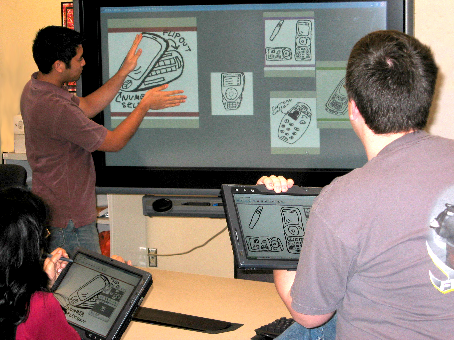
\includegraphics[width=\linewidth]{gfx/teamStormDisplayInteraction.png}
	\caption{Designer bei der Ausarbeitung von Konzepten mit \emph{Team Storm}. Einer der Benutzer steht vor dem großen Display und erläutert seinen Kollegen, wie das von ihm konzipierte Design funktioniert.}
	\label{fig:teamStormDisplayInteraction}
\end{figure}

Skizzen, die von einem Teilnehmer aus seinem privaten Arbeitsbereich in den gemeinsamen Bereich gezogen werden, befinden sich standardmäßig im >>Ausstellungsmodus<<. Das bedeutet, dass alle Designer die Zeichnung sehen, sie positionieren und skalieren, jedoch nicht verändern können. Sollte der Urheber der Skizze wünschen, dass Größe und Position von seinen Kollegen ebenfalls nicht verändert werden dürfen, so kann er den Zugriff sperren. Er kann die Zeichnung jedoch auch ganz freigeben, sodass nicht nur Skalierung und Position für die Kollegen veränderbar sind. Um eine Zeichnung vom gemeinsamen Bereich zu entfernen, zieht der Designer sie wieder zurück in seinen privaten Arbeitsbereich.

Designer können freigegebene Skizzen direkt auf der gemeinsamen Arbeitsfläche modifizieren, damit die anderen Teilnehmer die Änderungen >>live<< mitverfolgen können. Zusätzlich gibt es die Möglichkeit, sich eine private Kopie zu erstellen, die ohne Einsicht der anderen Teilnehmer editiert werden kann. Dadurch können Designs in mehreren Iterationen\footnote{In diesem Zusammenhang bezeichnet die \emph{Iteration} einen sich wiederholenden Zyklus.} editiert und verfeinert werden. Die unterschiedlichen Versionen, nebeneinander angereiht, zeigen die Evolution einer bestimmten Idee.

Die an \emph{Team Storm} durchgeführte Studie \citep{Hailpern:2007p113} zeigt, dass Designer, die das erste Mal mit dem System arbeiteten, einen sehr einfachen und direkten Zugang zu dieser Groupware fanden. Es wurden sehr viele Ideen generiert und die Teilnehmer nutzten sehr stark die Features zur Organisation der Konzepte und Designs. Unterschiedliche Charaktere brachten unterschiedliche Arbeitsweisen zum Vorschein: einige Designer teilten offen jeden ihrer gezeichneten Striche mit, während andere es bevorzugten, Skizzen erst im privaten Bereich anzufertigen, um sie selbst zu evaluieren bevor sie sie herzeigten.

Die Gruppen nutzten das System auf sehr individuelle Art und Weise. Während manche hauptsächlich gemeinsam an einzelnen Designs arbeiteten, zogen andere es vor, parallel an verschiedenen Konzepten zu arbeiten, die dann gemeinsam evaluiert wurden.

Neben diesen positiven Eindrücken, kristallisierten sich auch einige mögliche Optimierungen des Systems heraus. Die Designer wünschten sich, Konzepte in Gruppen zu organisieren, die sie dann als Einheit positioniert, skaliert und hergezeigt hätten. Die Navigation wurde von vielen bei steigender Anzahl von Skizzen als ineffizient empfunden. Das System sah nur Scrolling und Zooming vor, die Teilnehmer wünschten sich hier weitere Möglichkeiten. Zusätzlich kam das Bedürfnis auf, andere digitale Artefakte (z.B. Bilder und Webseiten) einzubinden und dadurch Skizzen anzureichern.

\section{Human and technical factors of distributed group drawing tools}
Greenberg et al. untersuchen in einer Studie \citep{Greenberg:1992p207} die menschlichen und technischen Faktoren, denen beim Design von multi-user Software hohe Relevanz zukommt. Sie haben für ihre Untersuchungen vier Systeme entwickelt (GroupSketch, XGroupSketch, GroupDraw und GroupKit), die kollaboratives Skizzieren in einer räumlich verteilten Gruppe ermöglichen. Beim Design dieser Applikationen, versuchte man sich möglichst genau an das deskriptive Framework von Tang (1989) \citep{TangJC:1989} zu halten, welches wir in einem späteren Kapitel noch genauer erörtern werden.\\ \color{red}TODO: Referenz zu späterem Kapitel einfügen.\\
\color{black}
\subsection{GroupSketch} 
GroupSketch ist ein simples, gruppenorientiertes Zeichentool. Es erlaubt einer beliebigen Anzahl von Benutzern, gemeinsam auf ein virtuelles Blatt Papier (dargestellt auf einem Monitor) zu zeichnen. Jeder Benutzer hat einen eigenen Computer, der mit den anderen Computern über ein Netzwerk verbunden ist, daher hat jeder eigene Ein- und Ausgabegeräte zur Verfügung.

Die Hauptfunktionen von GroupSketch sind die folgenden:
\begin{itemize}
	\item
	Umsetzung als WYSIWIS-Editor (What You See Is What I See), wodurch garantiert wird, dass jeder Benutzer zu jedem Zeitpunkt dasselbe auf seinem Monitor sieht, wie alle anderen.
	\item
	Jeder Teilnehmer hat einen eigenen Mauscursor, der immer für alle sichtbar und eindeutig identifizierbar ist. Dadurch sind simultane Eingaben möglich.
	\item
	Jegliche Benutzerinteraktion, so unwichtig sie auch erscheinen mag, ist sofort auf allen Bildschirmen sichtbar.
	\item
	Der Zugang zu unterschiedlichen Eingabemodi, sprich Zeichnen, Gestikulieren und das Anfügen von Notizen, ist so einfach und unkompliziert wie möglich. 
\end{itemize}

Jeder Cursor trägt den Namen seines Besitzers, damit immer klar ersichtlich ist, wer gerade was macht. Zusätzlich wird jeder Benutzer durch eine kleine Karikatur an der rechten Seite des Monitors dargestellt.

Es gibt vier verschiedene Interaktionsformen: mit dem Cursor zeigen, zeichnen, bzw. löschen und mit der Tastatur schreiben. Der Cursor spiegelt immer den aktuellen Modus wieder. Wenn keine Maus- oder Tastaturtasten gedrückt werden, nimmt er die Form einer zeigenden Hand an. Durch das Bewegen der Maus, kann ein Benutzer auf Dinge zeigen und simple Gesten durchführen. Zum Zeichnen verwendet man die linke Maustaste und zum Schreiben kann man einfach los tippen und GroupSketch platziert die Schrift an der aktuellen Position der Maus. Während des Zeichnens und Schreibens, verwandelt sich der Cursor von einer zeigenden Hand in einen Schreibstift. Durch Drücken der mittleren Maustaste wechselt das Bild des Cursors zu einem großen Pfeil, der dazu dient, die Aufmerksamkeit der anderen Benutzer zu erlangen. Die rechte Maustaste ermöglicht das Löschen von Zeichnungen und Notizen. 

\subsection{XGroupSketch}
XGroupSketch verfolgt ein ähnliches Konzept wie GroupSketch, unterscheidet sich aber deutlich in einigen wichtigen Punkten. Während GroupSketch immer im Vollbildmodus läuft, wird XGroupSketch in einem Fenster dargestellt. Dadurch hat verfügt jeder Benutzer über horizontale und vertikale Scrollbalken und streng genommen handelt es sich daher nicht mehr um einen WYSIWIS-Editor, denn es kann nicht gewährleistet werden, dass jeder zu jedem Zeitpunkt dasselbe sieht. XGroupSketch bietet gegenüber GroupSketch eine größere Palette an Funktionalität. Über mehrere Menüs können die Benutzer unterschiedliche Linienstärken, Farben und Schriften wählen, jedoch bedeutet dies, dass die Applikation weitaus komplizierter in ihrer Bedienung ist, als GroupSketch.

\subsection{GroupDraw}
Im Gegensatz zu den vorhergehenden zwei rasterbasierten Zeichenprogrammen, ist GroupDraw eine objektorientierte Applikation. Es werden ebenfalls mehrere Cursor unterstützt und Benutzer können außer Freihand auch Grundformen, wie Rechtecke, Kreise und Linien erstellen. Diese gelten als Objekte und können von allen Benutzern selektiert und positioniert werden. Auch bei GroupDraw wurde das strenge WYSIWIS-Konzept gelockert. Genauso wie XGroupSketch läuft die Applikation in einem Fenster und jeder Benutzer kann selbst bestimmen, welchen Teil der Zeichenfläche er sieht. Ein Vorteil dieser Methode ist, dass die Teilnehmer gleichzeitig und für sich, in verschiedenen Bereichen an eigenen Zeichnungen arbeiten können, ohne sich dabei in die Quere zu kommen. 

Das objektorientierte Konzept und die dadurch gewonnenen Möglichkeiten, ziehen eine erhebliche Anzahl an möglichen Konflikten mit sich. Bereits die Tatsache, dass Objekte von Benutzern selektiert und verändert werden können, erfordert Maßnahmen zur Tilgung von Konflikten, die auftreten können. So muss überlegt werden, was passieren soll, wenn zwei Benutzer gleichzeitig versuchen, das Objekt zu verändern. Die einfachste Methode ist jene, das Objekt sofort zu sperren wenn ein Benutzer Zugriff erhält, aber es muss auch eine sinnvolle Art der Visualisierung dieser Sperre gegenüber anderen Benutzern gefunden werden. Es wäre denkbar, dass das Objekt für jene Benutzer, die gerade keinen Zugriff darauf haben, halbtransparent dargestellt wird.

Das nahtlose Mischen von Arbeitsbereich, Aktionen und Funktionen, wie es von Tang \citep{TangJC:1989} empfohlen wird, ist in GroupDraw sehr schwierig umzusetzen. GroupSketch hat den Vorteil, dass es mit sehr wenig Funktionalität auskommt und der Zugang kann dadurch sehr simpel gestaltet werden. Durch die vielen verschiedenen Zeichenmöglichkeiten, die GroupDraw bietet, nimmt das grafische User Interface stark an Komplexität zu. Während es in single-user Applikationen nicht grundsätzlich problematisch ist, ein komplexeres Interface zu haben, kann es in multi-user Software eine erhebliche Einschränkung im Workflow der gesamten Gruppe bedeuten. 

GroupDraw verfügt über zwei Mechanismen, die dem Schutz der Privatsphäre innerhalb der Gruppe dienen. Einerseits können Benutzer sich einen eigenen Bereich zum skizzieren suchen und diesen erst nach persönlicher Evaluierung der Zeichnungen den anderen Teilnehmern zeigen. Andererseits können für jedes Objekt spezielle Berechtigungen vergeben werden. Ein Objekt kann von allen Teilnehmern gesehen und verändert werden, kann von allen gesehen aber nur vom Besitzer verändert werden, kann nur vom Besitzer gesehen und verändert werden.

\subsection{GroupKit}
GroupKit ist ein Toolkit zur Entwicklung von verteilter Echtzeit-Groupware. Obwohl Applikationen, die mit Hilfe von GroupKit entwickelt werden, auch für andere Szenarios als das bloße Zeichnen geeignet sind, waren die Erkenntnisse der zuvor vorgestellten Systeme sehr wichtig für das Design von GroupKit.

Die Praxiserfahrungen mit GroupSketch, XGroupSketch und GroupDraw zeigen, dass neben den von Tang definierten Designkriterien \citep{TangJC:1989} noch folgende Faktoren bei der Entwicklung von groupware Zeichenapplikationen von Bedeutung sind:

\begin{itemize}
	\item
	Die Notwendigkeit einer höheren Telepräsenz
	\item
	Die Möglichkeit nahtloser Übergänge zwischen lokalen, privaten Daten und gemeinsam erstellten Arbeiten zu bieten
	\item
	Berücksichtigung der Anzahl der Benutzer in der Gruppe
\end{itemize}

Die Recherchen \citep{Greenberg:1992p207} haben gezeigt, dass GroupSketch und GroupDraw während der Zusammenarbeit von räumlich distanzierten Gruppen eine ausreichend hohe Telepräsenz gewährleisten, solange Zeichnen und Skizzieren im Mittelpunkt der Konzeption stehen. Saß die Gruppe im selben Raum, so wandte sich die Aufmerksamkeit vom Computer ab und die Teilnehmer gingen über zu face-to-face Kommunikation, sobald die Skizzen nicht mehr zentrales Thema der Diskussion waren. 

Ferner weisen die Autoren \citep{Greenberg:1992p207} darauf hin, dass es zur Zeit der Untersuchungen (1992) noch zu hohe Barrieren zwischen virtuellen und realen Artefakten gibt. Im Zuge eines Meetings ist es nicht ohne weiteres möglich, echte Artefakte zu digitalisieren und mit anderen zu teilen.

Letztlich ist die Anzahl der Benutzer ein kritischer Faktor für die Art und Weise, wie eine gemeinsame Zeichenfläche genutzt wird. Die vorgestellten Systeme GroupSketch und GroupDraw funktionieren gut im Einsatz mit Gruppen die aus 2-4 Personen bestehen. Sehr häufig arbeiten aber weitaus mehr Menschen zusammen und es bleibt die Frage im Raum, ob die Systeme dementsprechend skalieren. Ein Test mit acht Teilnehmern hat bereits einige Problemstellen entlarvt. Das Konzept der multiplen Cursor kann sehr schnell dazu führen, dass der Bildschirm überfüllt wirkt und die vielen Bewegungen mögen etwas irritierend sein. Um diesem Phänomen entgegen zu wirken, verkleinern sich die Cursor entsprechend ihrer Anzahl. Wenn Benutzer bestimmte Aktionen durchführen, vergrößert sich der jeweilige Cursor während dessen wieder auf normale Größe, damit Interaktionen gut erkennbar bleiben. 

\section{Why CSCW applications fail: problems in the design and evaluation of organizational interfaces}

In seiner Studie über die Schwierigkeit des Designs und der Evaluierung von CSCW-Applikationen \citep{Grudin:1988p126}, nennt Jonathan Grudin drei grundlegende Problemfelder:

\begin{itemize}
	\item
	Das Missverhältnis zwischen denen, die einen zusätzlichen Aufwand betreiben müssen und jenen die einen tatsächlichen Nutzen haben
	\item
	Das Treffen von Entscheidungen durch leitende Personen, basierend auf ihrer Erfahrung und Intuition
	\item
	Das Unterschätzen der Schwierigkeiten, die mit einer Evaluierung von CSCW-Systemen verbunden sind
\end{itemize}

Am Beispiel einer Software zur automatischen Planung von Sitzungen zeigt Grudin wie ein ungleiches Verhältnis zwischen einzelnen Nutzern einer CSCW-Applikation entstehen kann. 

Wenn ein Mitarbeiter eine Sitzung mit anderen vereinbaren möchte, so muss er der Software nur die gewünschten Teilnehmer mitteilen. Das Programm vergleicht dann eigenständig die elektronischen Kalender dieser Personen und bucht einen Termin zu jener Zeit, in der noch alle Teilnehmer frei sind. Voraussetzung hierfür ist dementsprechend, dass jeder Mitarbeiter im Unternehmen einen elektronischen Kalender führt. Jene Personen, die in leitenden Positionen tätig sind, führen sehr wahrscheinlich einen Kalender oder haben eine Sekretärin, die diese Aufgabe übernimmt. Probleme ergeben sich dann, wenn leitende Mitarbeiter Termine mit Angestellten vereinbaren möchten, da diese häufig keinen elektronischen Kalender führen. Das System glaubt daher, dass ein Termin zu jeder Zeit möglich wäre und bucht unter Umständen einen ungünstigen Zeitpunkt für entsprechende Teilnehmer. Um dieser Problematik vorzubeugen, müssten alle Mitarbeiter, vom einfachen Angestellten bis hin zum Geschäftsführer, einen elektronischen Kalender führen. \graffito{CSCW Software muss so konzipiert werden, dass jeder User einen Nutzen hat und zusätzliche Aufwände so gering wie möglich ausfallen.} Angestellte hätten dadurch einen zusätzlichen Aufwand, jedoch wenig bis gar keinen Nutzen vom System. Dieser Umstand kann sehr leicht dazu führen, dass die Software in der Praxis keine Akzeptanz unter den Benutzern findet und dadurch scheitert.

\medskip Beim Design von multi-user Software verlassen sich laut Butler et al. \citep{ButlerK:1987} Entscheidungsträger häufig auf ihre Intuition, die wiederum auf persönlichen Erfahrungen, zumeist im single-user Bereich, beruht. Es mag relativ einfach sein, ein Gespür dafür zu entwickeln, wie gut die User-Experience\footnote{TODO: define User-Experience} eines Textverarbeitungs- oder Tabellenkalkulationsprogramm ausfällt, jedoch wird CSCW Software von einem breiten Spektrum an Personen verwendet und alle diese Benutzer haben unterschiedliche Hintergründe und Berufe, ungleiches technisches Know-How und abweichende Zugänge zum Programm. Die Software wird sehr wahrscheinlich scheitern, wenn die Intuition der Entscheidungsträger die durch solch eine Gruppendynamik zustande gekommene Komplexität ignoriert. 

Die von Grudin \citep{Grudin:1988p126} angeführte Software zur automatischen Planung von Sitzungen bezeichnet er selbst als anfällig für ein solches Scheitern durch falsche Intuition von leitenden Mitarbeitern. Er begründet dies so, dass jene leitenden Mitarbeiter selbst mit großer Wahrscheinlichkeit bereits einen elektronischen Kalender führen und daher vordergründig nur den eigenen Nutzen erkennen. Mangelnde Empathie kann zu Folge haben, dass der zusätzliche Aufwand, der einfachen Angestellten entsteht, nicht berücksichtigt wird. 

\medskip Die Evaluierung von CSCW Software erfordert eine spezielle Vorgangsweise, basierend auf den Methoden der Psychologie und Anthropologie \citep{Grudin:1988p126}. Laut Grudin fehlen diese Fähigkeiten zum Zeitpunkt der Untersuchung (1988) in den meisten Entwicklungs- und Forschungsteams, da qualifizierte Personen aus den Bereichen \emph{Human Factors Engineering}\footnote{Als \emph{Human Factors Engineering} bezeichnet man jene Disziplin, die sich mit den Fähigkeiten und Grenzen des Menschen beschäftigt und diese Erkenntnisse auf das Design von Produkten, Prozessen, Systemen und Arbeitsplätzen anwendet. Dazu gehört das Überprüfen auf \emph{Usability}, das Erstellen von Nutzerprofilen und die Entwicklung von Benutzerdokumentation und Trainingsprogrammen.} und kognitiver Psychologie noch selten vertreten sind. Zusätzlich ist der mit der Evaluierung verbundene zeitliche und finanzielle Aufwand erheblich höher, da immer ganze Gruppen an Probanden getestet werden müssen.

\section{Concepts that Support Collocated CSCW}
Auf der Suche nach Konzepten, zur Förderung der kreativen Zusammenarbeit von Industriedesigner in gemeinsamen Meetings, halten Wang und Blevis \citep{Wang:2004p110} sich an die Methode des \emph{human centered design}\footnote{Beim \emph{human centered design} steht der potenzielle Benutzer eines Produktes im Mittelpunkt des Entwicklungsprozesses. Seine Aufgaben, Ziele, Fähigkeiten und Eigenschaften werden analysiert und gelten als Maßstab bei der Gestaltung des Produkts. \emph{Human centered design} zielt darauf ab, möglichst benutzerfreundliche Produkte zu schaffen.} und führen zuerst eine ethnographische Studie an der Zielgruppe durch. Ausgehend von den so erlangten Erkenntnissen, entwickeln sie vier unterschiedliche Konzepte, die speziell darauf abzielen, die konkrete Arbeitsweise der Industriedesigner zu unterstützen. Diese Konzepte sind aus technischer Sicht nicht unbedingt innovativ, dafür aber für ihre Zielgruppe besonders gut geeignet.

In ihrer Studie konzentrieren sich Wang und Blevis \citep{Wang:2004p110} darauf, die Interaktionen zwischen den Designern zu beobachten und nicht die Interaktion mit speziellen interaktiven Geräten. Ferner observieren die Forscher die verschiedenen nicht technologischen Artefakte und Geräte, sowie deren Orientierung und Gebrauchsweise, die bei der Zusammenarbeit zum Einsatz kommen. Davon ausgehend versuchen sie, möglichst ganzheitliche Konzepte zu entwickeln. Den letzten Fokus der Studie bildet das Identifizieren der Unterschiede zwischen privaten und gemeinsamen Arbeitsbereichen im kollaborativen Prozess.

Die folgenden relevanten Punkte haben sich aus dieser Studie heraus kristallisiert und fließen als Designkriterien in die danach vorgestellten Konzepte mit ein.

\begin{itemize} 
	\item{\emph{Sitzordnung}}\\
	Augenkontakt ist eine der wichtigsten Formen der Kommunikation bei der Zusammenarbeit in Gruppen. Daher bevorzugen die Teilnehmer, um einen Tisch herum zu sitzen, damit sie alle direkt ansehen können.
	\item{\emph{Reichweite}}\\
	Es ist besonders wichtig, dass alle Objekte für jeden Teilnehmer in Reich- und Sichtweite liegen. Durch die Interaktion mit den Objekten, können Teilnehmer sich in den Fokus der Aufmerksamkeit bringen und besser kommunizieren. Rechteckige Tische bieten Nachteile für jene Personen, die an den Ecken sitzen, weshalb runde Tische bevorzugt werden.
	\item{\emph{Simultanität}}\\
	Häufig interagieren mehrere Benutzer gleichzeitig mit den Objekten im Arbeitsbereich und fast immer sind viele verschiedene Artefakte präsent. Ein gutes Konzept muss daher diese Gleichzeitigkeit gewährleisten können, um die Effizienz durch paralleles Arbeiten nicht zu gefährden.
	\item{\emph{Gebrauch physischer Objekte}}\\
	In der direkten face-to-face Kommunikation bevorzugen Personen physische Objekte, da sie im Gespräch effizienter genutzt werden können als digitale Objekte.
	\item{\emph{Große Arbeitsflächen, viele Blätter, Wiederfindung und Vergleich}}\\
	Designer benötigen sehr große Arbeitsflächen im Zuge der kreativen Ideenfindung. Sie verteilen die verschiedenen Konzepte darauf und Anordnung und Gruppierung spielen eine wichtige Rolle. Um einzelne Ideen leichter wieder zu finden und untereinander zu vergleichen, zeichnen sie üblicherweise nur eine davon auf ein gesamtes Blatt Papier.
	\item{\emph{Privatsphäre}}\\
	Die Teilnehmer benötigen private Arbeitsbereiche, in denen sie Konzepte ausarbeiten und selbst evaluieren können, und sie brauchen gemeinsame Arbeitsbereiche, auf denen sie alle zusammen die Entwicklung vorantreiben.
	\item{\emph{Ausrichtung von Objekten}}\\
	Die Ausrichtung von Objekten ist Teil der Privatsphäre. Sind Objekte zu einer bestimmten Person hin ausgerichtet, so gelten diese als privat, wenn sie hingegen zur Gruppe hin gerichtet sind, finden alle Teilnehmer einen Zugang.
\end{itemize}





%*****************************************
%*****************************************
%*****************************************
%*****************************************
%*****************************************
